\section{Construction of Vietoris-Rips complexes} \label{sec:computing-complexes}
\label{sec:vietoris-rips-construction}

We dedicate this section to the problem of constructing the Vietoris-Rips filtration of a given metric space. We first introduce the problem formally. 

\begin{problem}[VRFilt]
Instance: let $(M,d)$ be a metric space and $S \subset M$ be a finite set of points. \\
Question: compute a compatible ordering of simplices from the filtered Vietoris-Rips complex $(\vr(S; \varepsilon))_{\varepsilon \in \R_{\geq 0}}$.
\end{problem}

For a metric space $(M, d)$, $S \subset M$, we note that $K = \vr(S; \infty)$ is the simplicial complex containing a single $\lvert S \rvert$-simplex and all of its faces, so the total count of faces is the sum of the first $n$ triangular numbers (including the zeroth triangular number), which is not computationally feasible. It is for this reason that we upper bound $\varepsilon$ in our construction, giving the following derived problem.

\begin{problem}[$\hat\varepsilon$-VRFilt]
Instance: let $(M,d)$ be a metric space, $S \subset M$ be a finite set of points, and $\hat\varepsilon \in \R_{\geq 0}$. \\
Question: compute a compatible ordering of simplices from the filtered Vietoris-Rips complex $(\vr(S; \varepsilon))_{\varepsilon \in [0, \hat\varepsilon]}$.
\end{problem}

We now follow the approach given by \textcite{zomorodian2010fast}. Let $(M,d)$ be a metric space, $S \subset M$ be a finite set of points, and $\hat\varepsilon \in \R_{\geq 0}$. We may split the computation of the Vietoris-Rips complex into the following phases:
\begin{enumerate}
    \item compute the weighted graph $(G, w)$ where $G = (V,E)$ is the $1$-skeleton of $\vr(S; \hat\varepsilon)$ and $w: E \to \R_{\geq 0}$ is defined by $w(u,v) = d(u,v)$;
    \item compute the \emph{expansion} of $(G, w)$ to the weight-filtered simplicial complex $(\vr(S; \hat\varepsilon), w)$; then
    \item obtain the simplex ordering by sorting the simplices according to their weights.
\end{enumerate}

Let $n$ be the number of points in $S$. We assume that we can compute $d(u,v)$ for any $u, v \in S$ in $O(1)$ time. It is clear \text{(iii)} reduces to \textsc{Sorting}, which we can achieve in time $\Theta(n\log n)$. Thus, we bring our focus to (i) and (ii), algorithms for which will be hence force referred to as the \emph{skeleton method} and \emph{expansion method} respectively.

\subsection{Skeleton methods}

We first formalise the skeleton method, which reduces to the following problem.

\begin{problem}[$\varepsilon$-NNs]
Instance: let $(M, d)$ be a metric space, $S \subset M$ be a finite set of points, and $\varepsilon \in \R_{\geq 0}$. \\
Question: for each $x \in S$, compute $\{y \in S \setminus \{x\}: d(x,y) \leq \varepsilon\}$.
\end{problem}

\textsc{$\varepsilon$-NNs} has the following approximate analogue.

\begin{problem}[$(1 + \delta, \varepsilon)$-ANNs]
Instance: let $(M, d)$ be a metric space, $S \subset M$ be a finite set of points, and $\varepsilon \in \R_{\geq 0}$. \\
Question: for each $x \in S$, compute $\{y \in S \setminus \{x\}: d(x, y) \leq (1 + \delta) \varepsilon\}$.
\end{problem}

We first recognise the brute-force solution, which may run in $O(n^2)$ time and has the benefit of being exact.

\textcite{arya1998optimal} made use of a particular tree structure (called BBD-trees) to achieve a solution in the case when $M = \R^d$, with query time of $O(c(d) \log n)$ and $O(dn)$ space, with $O(dn\log n)$ processing time. The function $c(d)$ is some function dependent on the dimension of $M$, there is no information on the asymptotic behaviour of this function presented in the literature, but empirical evidence suggests that it depends heavily on the underlying distribution of $S \subset M$.

The exact algorithm provided by \textcite{arya1998optimal} is in fact an approximation algorithm that allows the value of $\delta$ to be set (precisely to $\delta = 0$ for the exact case). In the case $\delta > 0$, the function $c$ given above also depends on $\delta$ but all other complexities remain the same. A lower bound of $c$ is given as
\[c(d, \delta) \leq d \lceil 1 + 6d/\delta \rceil^d. \]

% \subsubsection{Randomised algorithms for (i)}

% Both algorithms above suffer from the \emph{curse of dimensionality}; that is, when $M = \R^d$, $d$ heavily effects the running time of algorithms, leading to intractable solutions for high dimensions (more than 20).

A recent benchmark study \cite{aumuller2020ann} found the fastest current algorithm to solve \textsc{$(1 + \delta, \varepsilon)$-ANN} as one based on \emph{navigable small-world graphs with controllable hierarchy} \cite{malkov2018efficient}. We briefly touch on some underlying theory before introducing this algorithm.

A graph is a \emph{navigable small-world graph} if the greedy graph routing (shown in Algorithm \ref{alg:nearest-neighbour-greedy-routing}) runs in $O(\log^k n)$ time, for $k > 1$. We combine such a graph with the concept of \emph{skip lists}.

\begin{algorithm}
    \caption{A greedy routing algorithm for \textsc{$\varepsilon$-NNs}.}
    \label{alg:nearest-neighbour-greedy-routing}
    \begin{algorithmic}[1]
        \Function{GreedyRouting}{graph $G$, heuristic $h$, start node $v$}
        \State $\text{best} \gets v$
        \While{true}
        \State $\text{bestNeighbour} \gets \argmax_{n \in N_G(\text{best})} h(n)$
        \If{$h(\text{bestNeighbour}) > h(\text{best})$}
        \State $\text{best} \gets \text{bestNeighbour}$
        \Else
        \State \Return best
        \EndIf
        \EndWhile
        \EndFunction
    \end{algorithmic}
\end{algorithm}

A \emph{skip list} is a probabilistic data structure that allows $O(\log{n})$ average search complexity and insertion complexity within an ordered sequence of $n$ elements.

The initial idea: for a sorted list, we create a duplicate list where a given element of the initial list is duplicated with probability $0.5$. For every duplicated item, we store a pointer at the item in the second list back to the first list. We also add \emph{sentinel nodes} for safety. We do this for the sorted list $(0,1,2,3,4,5,6)$ as follows.

\begin{center}
    \begin{tikzcd}
        -\infty \arrow[r] & 0 \arrow[d] \arrow[r] & 1 \arrow[rr] \arrow[d]
        && 3 \arrow[d] \arrow[rrr] &&& 6 \arrow[d] \arrow[r] & \infty \\
        -\infty \arrow[r] & 0 \arrow[r] & 1 \arrow[r] & 2 \arrow[r]
        & 3 \arrow[r] & 4 \arrow[r] & 5 \arrow[r] & 6 \arrow[r] & \infty
    \end{tikzcd}
\end{center}

Searching for $5$ is shown below.

\tikzset{emph/.style={preaction={ % allow highlighting
                    draw,blue!25,-, double=blue!25, double distance = 8\pgflinewidth
                }}}

\begin{center}
    \begin{tikzcd}
        -\infty \arrow[r, emph] & 0 \arrow[d] \arrow[r, emph]
        & 1 \arrow[rr, emph] \arrow[d]
        && 3 \arrow[d, emph] \arrow[rrr] &&& 6 \arrow[d] \arrow[r] & \infty \\
        -\infty \arrow[r] & 0 \arrow[r] & 1 \arrow[r] & 2 \arrow[r]
        & 3 \arrow[r, emph] & 4 \arrow[r, emph] & 5 \arrow[r]
        & 6 \arrow[r] & \infty
    \end{tikzcd}
\end{center}

The probability a given duplicated node is followed by $k$ non-duplicated nodes is $\frac1{2^k}$. Thus, the expected number of nodes examined when searching the initial list is $\sum_{k = 1}^\infty \frac1{2^k} = 2$. So by adding this \emph{shortcut list}, we have reduced the expected time complexity
from $n$ to $\frac n2 + O(1)$.

An improvement: keep adding shortcut lists of the top shortcut list until we are out of elements.

\begin{center}
    \begin{tikzcd}
        -\infty \arrow[rrrrrrrr] \arrow[d] & & & & & & & & \infty \arrow[d] \\
        -\infty \arrow[rr] \arrow[d] & & 1 \arrow[rrrrrr] \arrow[d] & & & & &
        & \infty \arrow[d] \\
        -\infty \arrow[rr] \arrow[d] & & 1 \arrow[rrrrr] \arrow[d]  & & & &
        & 6 \arrow[r] \arrow[d] & \infty \arrow[d] \\
        -\infty \arrow[r] \arrow[d] & 0 \arrow[r] \arrow[d]
        & 1 \arrow[rr] \arrow[d] & & 3 \arrow[rrr] \arrow[d] & &
        & 6 \arrow[r] \arrow[d] & \infty \arrow[d] \\
        -\infty \arrow[r] & 0 \arrow[r] & 1 \arrow[r] & 2 \arrow[r]
        & 3 \arrow[r] & 4 \arrow[r] & 5 \arrow[r] & 6 \arrow[r] & \infty
    \end{tikzcd}
\end{center}

The expected number of levels is $\log{n}$, which is easy to prove. At each level, we cut search time in half (excluding overhead, which we assume is $O(1)$). This gives us a search time of $O(\log{n})$.

To combine this with navigable small-world networks: we build layers of graphs up sequentially. The bottom layer (as in skip lists) is the graph where the vertices are our points and two points have an edge if they are an $\varepsilon$-neighbour. Vertices have a fixed probability of moving up to the next layer, and the way we choose neighbours in higher layers is by using a heuristic that favours diverse connections.

Hierarchical navigable small-world networks are a relatively new technique for nearest neighbour search, and as such has found little application to problems such as persistent homology. We emphasise this as a material for further research, comparing its use for Vietoris-Rips construction against other established techniques. We will not cover any more of this algorithm here. 


\subsection{Expansion methods}

Methods presented here are introduced by \textcite{zomorodian2010fast}, as well as the complexity analysis. 

The expansion of a 1-skeleton effectively \emph{fills in} higher dimensional simplices whose faces are present, and assigns a weight to these simplices. That is, for a graph $G$, calculate the clique complex $\Cl(G)$ with a corresponding weight function $w: \Cl(G) \to \mathbb R_{\geq 0}$. 

We have seen that we can easily compute the weights on the simplices (Lemma \ref{lem:weight-definition-equivalent}), thus we focus on the construction of the clique complex.

\begin{problem}[CliqueComplex]
    Instance: let $G = (V,E)$ be a graph. \\
    Question: compute $\Cl(G)$. 
\end{problem}

We are now discarding all embedding information of $S$, and focusing solely on the topological features of the $1$-skeleton given by the skeleton method. 

We first introduce the \emph{inductive expansion algorithm}. We fix some arbitrary ordering on the vertices of our 1-skeleton, to give meaning to the \textsc{LowerNghbrs} function in Algorithm \ref{alg:inductive-algorithm}.

\begin{algorithm}
    \caption{The inductive expansion algorithm.}
    \label{alg:inductive-algorithm}
    \begin{algorithmic}
        \Function{LowerNghbrs}{graph $G$, vertex $u \in G$}
        \State \Return $\{v \in V(G): v < u, \{u,v\} \in E(G)\}$
        \EndFunction
        \Function{InductiveExpansion}{graph $G$, level $k \in \{2, 3, \ldots\}$}
        \State $K \gets V(G) \cup E(G)$
        \For{$i \gets 1$ to k}
        \For{each $i$-simplex $\tau \in K$}
        \State $N \gets \cap_{u \in \tau} \textsc{LowerNghbrs}(G, u)$
        \For{each $v \in N$}
        \State $K \gets K \cup \{\tau \cup \{u\}\}$
        \EndFor
        \EndFor
        \EndFor
        \EndFunction
    \end{algorithmic}
\end{algorithm}

We briefly share some intuition of Algorithm \ref{alg:inductive-algorithm} (a sketch of correctness): the skeleton of this code follows closely to the brute force method. For each $i$-simplex, we check if it forms the face of a $(i+1)$-simplex (using the fixed ordering to avoid double checking simplices). If it does, we add that $(i+1)$-simplex to the complex.

Analysing the complexity of expansion algorithms is tricky as we have an output that has exponential size (in the size of the input), but we can form a rough lower bound on the first level of expansion: from line segments to triangles. For each edge, we look at the (lower) neighbours of the endpoints to compute the set of shared (lower) neighbours. We then perform a constant time operation on each of the shared neighbours, thus we get the lower bound $\sum_{v \in V} \left(\deg v\right)^2$. This was was bounded by \textcite{de1998upper}:
\[
    \frac{4\lvert E \rvert^2}{\lvert V \rvert} \leq \sum_{v \in V} \left(\deg v\right)^2 \leq \lvert E \rvert \left(
    \frac{2\lvert E \rvert}{\lvert V \rvert - 1} + \lvert V \rvert - 2
    \right).
\]
Thus, the first level of expansion runs in time $O(n^3)$. We repeat the subsequent levels by a similar sum on the degrees on the triangles, tetrahedron, etc.; however, we typically fix the number of dimensions to expand into, so we take the overall time complexity to be $O(n^3)$. Further research is needed into the restriction of this bound.

We highlight a key inefficiency in the inductive algorithm (to motivate the incremental algorithm): when we compute the neighbours of a simplex, we repeat computations already done for its faces. Thus, instead of inducting on dimension, we can incrementally add vertices and construct cofaces for which the vertex is maximal. 

\begin{algorithm}
    \caption{The incremental expansion algorithm, where we induct on the dimension.}
    \label{alg:incremental-algorithm}
    \begin{algorithmic}
        \Function{AddCofaces}{graph $G$, level $k$, simplex $\tau$, $N$, $K$}
        \If{$\dim\tau \geq k$}
        \State \Return
        \EndIf
        \For{each $v \in N$}
        \State $\sigma \gets \tau \cup \{v\}$
        \State $M \gets N \cap \textsc{LowerNghbrs}(G, v)$
        \State $\textsc{AddCofaces}(G, k, \sigma, M, K)$
        \EndFor
        \EndFunction
        \Function{IncrementalExpansion}{$G$, $k$}
        \State $K \gets \varnothing$
        \For{each $u \in V(G)$}
        \State $N \gets \textsc{LowerNghbrs}(G, u)$
        \State $\textsc{AddCofaces}(G, k, \{u\}, N, K)$
        \EndFor
        \EndFunction
    \end{algorithmic}
\end{algorithm}

In Algorithm \ref{alg:incremental-algorithm}, we start with an empty complex. We than add all the cofaces of each vertex for which the vertex is maximal. The initial calls of \textsc{AddCofaces} in \textsc{IncrementalExpansion} will add all simplices (of the $k$-skeleton) for which $u$ is a maximal vertex. 

Further restriction of the worst-case running time (than the one presented for the inductive algorithm) is yet to be seen. 

\subsection{Comparison of methods}

As discussed above, computing worst-case running time bounds is difficult for both expansion methods. Thus, we empirically examine the running time of the methods presented. 

We first introduce the dataset we will use to compare the methods outlined above: the noisy unit circle (NUC) with fluctuation $\alpha$. Points are taken uniformly at random from the annulus with outer radius $1 + \alpha/2$ and inner radius $1 - \alpha/2$ (we will take $\alpha = 0.1$ unless otherwise stated). The underlying population of this test set is homeomorphic to the open cylinder $S^1 \times (0,1)$.

Three experiments were conducted on an instance of NUC to investigate the performance of the methods outlined above for \textsc{$\hat\varepsilon$-VRFilt}:
\begin{enumerate}
    \item investigating the running time of the brute force skeleton method and the method provided by sklearn \cite{scikit-learn} with varying point count;
    \item investigating the running time of the three expansion methods with varying $\hat\varepsilon$; and
    \item investigating the running time of the two (non-brute force) expansion methods with varying $\hat\varepsilon$.
\end{enumerate}

For experiment (i), we take $\hat\varepsilon = 0.01$. Note that the method provided by sklearn does not use the state-of-the-art hierarchical navigable small-world networks. In fact, it does not use a single method. The package will scan the underlying dataset and pick the optimal algorithm, one possible algorithm uses BBD-trees as mentioned from \textcite{arya1998optimal}. For experiments (ii) and (iii) our test set consists of 1000 points and we calculate expansion up to 10 dimensions. 

\begin{figure}
    \makebox[\textwidth][c]{
        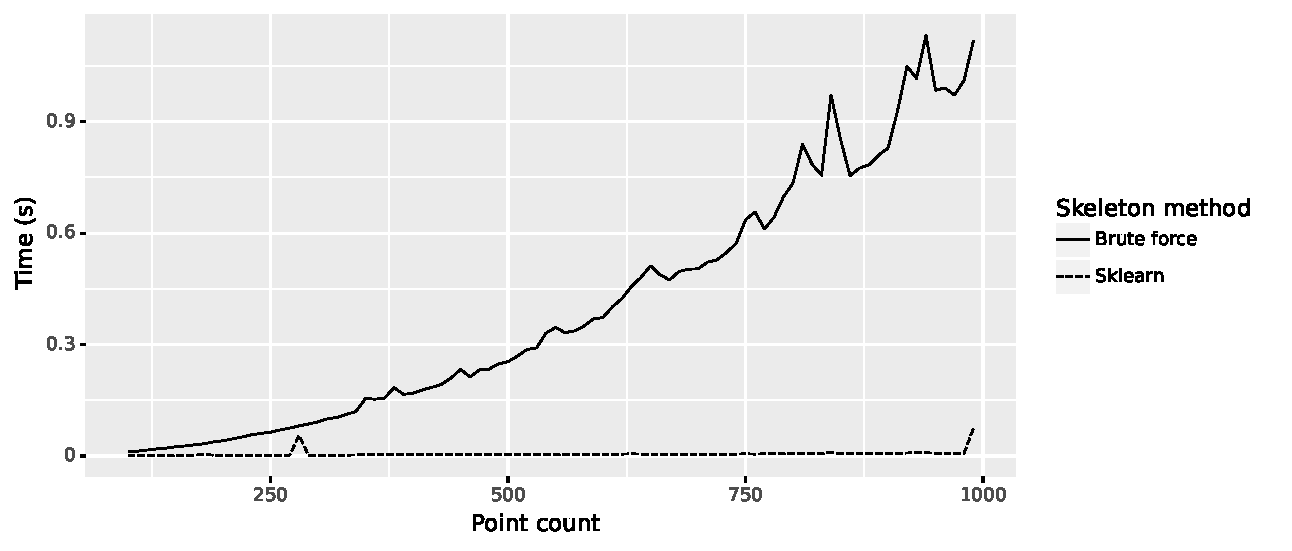
\includegraphics[width=1.2\textwidth]{content/4-comp-top/images/1-skeleton-methods}
    }
    \caption{A plot of the performance of two skeleton methods (with varying point count): the brute force method and the method provided by sklearn. The test set is the noisy unit circle (with radius fluctuation 0.1) with $\varepsilon = 0.01$.}
    \label{fig:skeleton-methods}
\end{figure}

Figure \ref{fig:skeleton-methods} shows the results of experiment (i), and we can clearly see that the brute force methods has poor performance. This figure does not show the performance of the sklearn method at higher point counts: the sklearn method (typically) runs in under a second for test sets of size \num{1000000} and higher (depending on $\hat\varepsilon$). From this, it is reasonable to conclude that the expansion method is the bottleneck in calculating the Vietoris-Rips filtration (the subsequent experiments reaffirm this claim).

\begin{figure}
    \makebox[\textwidth][c]{
        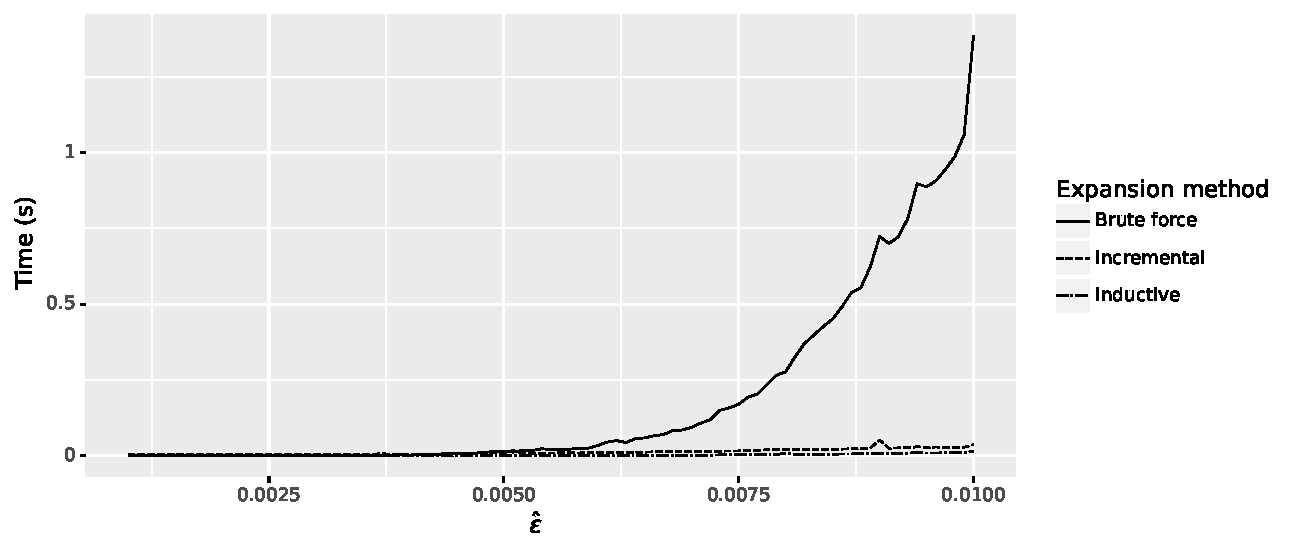
\includegraphics[width=1.2\textwidth]{content/4-comp-top/images/1-initial-expansion-methods}
    }
    \caption{A plot of the performance of three expansion methods (with varying $\varepsilon$): the brute force method, the inductive algorithm, and the incremental algorithm. The test set is is the noisy unit circle (with radius fluctuation 0.1) and the expansion is calculated up to 10 dimensions.}
    \label{fig:initial-expansion-methods}
\end{figure}

Figure \ref{fig:initial-expansion-methods} shows the results of experiment (ii), and reaffirms what the reader may expect: brute force algorithms are not very efficient. It is interesting to note that, at the range of $\hat\varepsilon$ plotted here, the inductive algorithm has better performance than the incremental algorithm (although they are similar).

\begin{figure}
    \makebox[\textwidth][c]{
        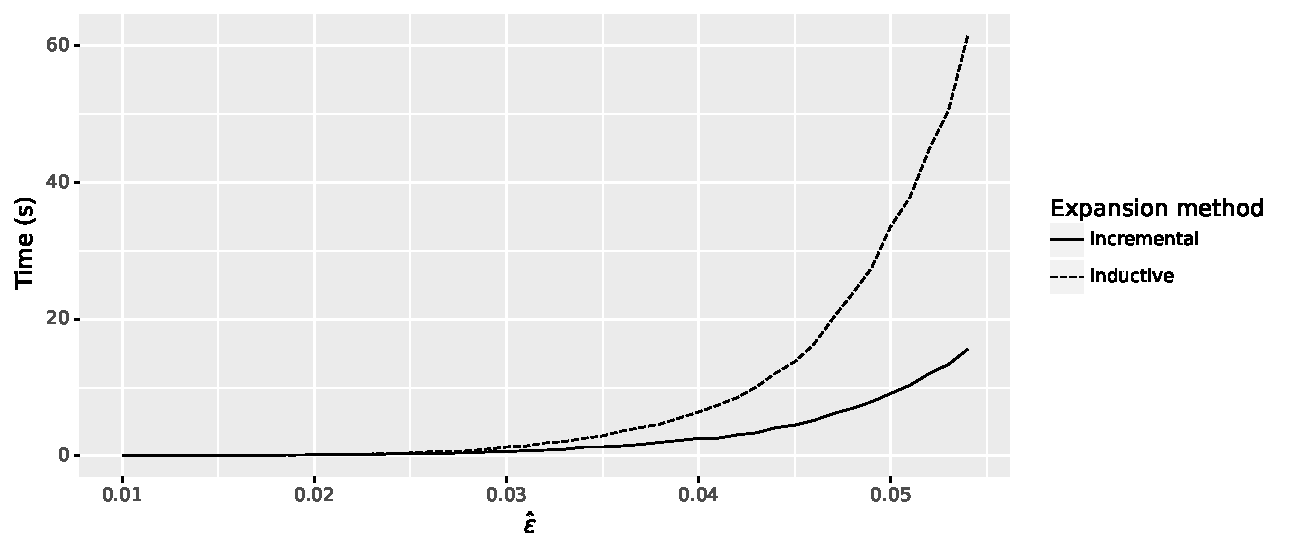
\includegraphics[width=1.2\textwidth]{content/4-comp-top/images/1-expansion-methods}
    }
    \caption{A plot of the performance of two expansion methods (with varying $\varepsilon$): the inductive algorithm and the incremental algorithm. The test set is is the noisy unit circle (with radius fluctuation 0.1) and the expansion is calculated up to 10 dimensions.}
    \label{fig:expansion-methods}
\end{figure}

Figure \ref{fig:expansion-methods} shows the results of experiment (iii) and shows that the incremental algorithm outperforms the inductive algorithm significantly, even though we saw the inductive algorithm perform slightly better for lower values of $\hat\varepsilon$.

To conclude, the incremental algorithm is the best investigated algorithm for expansion, and the sklearn methods outperform the brute-force solution. We again highlight the need for further research investigating hierarchical navigable small-world networks in this context. 

% \begin{definition}[Clustering coefficient]
%     Let $G$ be an undirected graph. The \emph{local clustering coefficient} of a vertex $v \in V(G)$ is given as
%     \[ C_G(v) = \frac{2 \lvert E(N_G(v)] \rvert}{\deg{v} (\deg{v} - 1)}. \]
%     The \emph{network average clustering coefficient} of $G$ is the average local clustering coefficients over all of the vertices in $G$:
%     \[ \overline C_G = \frac1{\lvert V(G) \rvert} \sum_{v \in V} C_G(v). \]
% \end{definition}

% We introduce the graph property of \emph{small-worldness}: a graph $G = (V,E)$ may be described as a \emph{small-world graph} if for each $u, v \in V$, $\E[d(u,v)] \propto \log^k{\lvert V \rvert}$ for some $k > 1$ and the network average clustering coefficient is not small. This concept is not particularly formal, and we will not formalise it here. However, there have been attempts to measure this property. In particular, \textcite{neal2015making} suggested a measure called the \emph{small-world index}, which we will denote by $\swi_G$. Conceptually, this measure evaluates:
% \begin{enumerate}
%     \item whether the average path length in $G$ is close to that of a random network with the same size and degree distribution (see \cite{erdos1959pmd} for details on this construction); and
%     \item whether the network average clustering coefficient of $G$ is close to that of a lattice network with the same size and degree distribution.
% \end{enumerate}
% It is noted that $\swi_G \in [0,1]$, with $\swi_G$ when $G$ does not have a small-world structure and $\swi_G = 1$ when $G$ has a small-world structure (although this is a theoretical maximum, construction of such a graph has not been seen).

% Let $G = (V,E)$ be an undirected graph and $\gr_G: V^2 \to \N_0$ be such that for $u, v \in V$, $\gr_G(u,v)$ denotes the length of a path from $u$ to $v$ as given by a greedy routing algorithm.
